% This is LLNCS.DEM the demonstration file of
% the LaTeX macro package from Springer-Verlag
% for Lecture Notes in Computer Science,
% version 2.3 for LaTeX2e



\documentclass{llncs}


\usepackage{ngerman}
\usepackage[T1]{fontenc}
\usepackage[utf8]{inputenc}
\usepackage{makeidx}  % allows for indexgeneration
\usepackage{multirow}
\usepackage{rotating}
\usepackage{verbatim}
\usepackage{graphicx}
\usepackage{float}
\usepackage{graphicx}  % For \resizebox
\usepackage{amssymb}   % AMS-Sonderzeichen
\usepackage{tabularx}  % Für tabularx und newcolumntype
\usepackage[paper=a4paper,left=25mm,right=25mm,top=25mm,bottom=25mm]{geometry}
\usepackage{array}
\usepackage{makecell}
\usepackage{color}
\usepackage{ragged2e}
\usepackage{longtable}
\usepackage{ifpdf}
% \usepackage{titlesec}
\usepackage{xcolor}    % Lieber xcolor als color. Dann klappt auch das listings gut mit den Farben
\usepackage{listings}
\usepackage{upquote}   % Verändert die Ausgabe der einfachen Anführungszeichen innerhalb von verbatim
\usepackage{eurosym}   % Euro-Zeichen: \euro
\usepackage{lastpage}  % \pageref{LastPage} um die Anzahl der Seiten zu erhalten
% hiermit kann man auch umlaute copy-pasten
\usepackage{lmodern}
\selectlanguage{english}
\usepackage{fancyhdr}
\usepackage{url}
\usepackage{caption}
\usepackage{float}
\setlength{\abovecaptionskip}{0pt} % Reduce space above the caption
\setlength{\belowcaptionskip}{0pt} % Space between caption and table
\captionsetup[table]{skip=5pt} % Adjust the value of '10pt' as needed
\pagestyle{fancy}
% Reduce space between float and surrounding text
\setlength{\textfloatsep}{0pt}
\setlength{\floatsep}{0pt}
\setlength{\intextsep}{0pt}



%

\ifpdf
\pdfinfo{
 /Author (Wladymir Alexander Brborich Herrera)
 /Author (Vishwaben Pareshbhai Kakadiya)
 /Author (Hellyben Bhaveshkumar Shah)
 /Author (Heer Rakeshkumar Vankawala)
 /Author (Priyanka Dilipbhai Vadiwala)
 /Title  (LowTech GMmBH Techincal Transformation Milestone 2)
 /Subject (Cloud Computing)
 /Keywords (Cloud Computing, Technical Transformation, Migration)
}
\fi

\setlength{\parindent}{0pt}    % Erste Zeile eines Absatzes nicht einrücken
\parskip2ex                    % Absatzabstand
\setlength{\itemsep}{0ex plus0.2ex}
\sloppy                        % Auf jeden Fall die Seitenränder einhalten.

\newcommand{\what}{Milestone 2: LowTech GMmBH Migration to Azure}
\newcommand{\who}{Group 23}
\newcommand{\when}{WiSe 2024-2025}

\renewcommand{\headrulewidth}{0.4pt}
\renewcommand{\footrulewidth}{0.4pt}
\lhead[\when]{\who}
\rhead[\who]{\when}
\chead[]{}
\lfoot[Page \thepage\ of \pageref{LastPage}]{\what}
\rfoot[\what]{Page \thepage\ of \pageref{LastPage}}
\cfoot[]{}
\pagestyle{fancy}


% Hurenkinder und Schusterjungen komplett verbieten.
\clubpenalty = 10000 
\widowpenalty = 10000 
\displaywidowpenalty = 10000
% Diese Begriffe bezeichnen den Makel beim Textsatz, wenn eine Seite mit der ersten Zeile eines Absatzes endet (so genannter Schusterjunge) oder eine neue Seite mit der letzten Zeile eines Absatzes beginnt (so genanntes Hurenkind).


% Wir definieren ein paar Farben
\definecolor{Brown}{cmyk}{0,0.81,1,0.60}
\definecolor{OliveGreen}{cmyk}{0.64,0,0.95,0.40}
\definecolor{CadetBlue}{cmyk}{0.62,0.57,0.23,0}
\definecolor{lightlightgray}{gray}{0.9}
\definecolor{FrankfurtBlue}{HTML}{3333b2}

% Hier fängt das Dokument an!
\begin{document}

%
% \frontmatter          % for the preliminaries
%
% \tableofcontents
%
\mainmatter              % start of the contributions
%
\title{\what}
%
\author{
    Wladymir Alexander Brborich Herrera (1437876)\\
    \texttt{wladymir.brborich-herrera@stud.fra-uas.de}
    \and\\
    Vishwaben Pareshbhai Kakadiya (1471845)\\
    \texttt{vishwaben.kakadiya@stud.fra-uas.de}
    \and\\
    Hellyben Bhaveshkumar Shah (1476905)\\
    \texttt{hellyben.shah@stud.fra-uas.de}
    \and\\
    Heer Rakeshkumar Vankawala (1449039)
    \\
    \texttt{heer.vankawala@stud.fra-uas.de}
    \and\\
    Priyanka Dilipbhai Vadiwala (1481466)\\
    \texttt{priyanka.vadiwala@stud.fra-uas.de}
}
%
\institute{
    Frankfurt University of Applied Sciences\\
    (1971-2014: Fachhochschule Frankfurt am Main)\\
    Nibelungenplatz 1\\
    D-60318 Frankfurt am Main\\
}

\maketitle              % typeset the title of the contribution

\begin{abstract}
    This report presents a comprehensive cloud transformation strategy for LowTech GmbH, developed by consultants from Awesome Cloud AG.
    Building on previous technical analyses, it outlines a strategic migration plan for the expanded application landscape,
    incorporating diverse service models such as IaaS, PaaS, and SaaS. The strategy identifies suitable public, private,
    and hybrid cloud environments to optimize performance and security while detailing operational cost calculations
    for a selected public cloud service provider. Key considerations include SAP requirements, legacy system maintenance,
    and leveraging DevOps and Cloud Native approaches for applications like the Webshop.
    The report critically analyzes the proposed solutions, balancing benefits and challenges,
    and aligning them with LowTech GmbH’s business objectives. This forward-looking strategy ensures scalability, flexibility, and resilience, positioning
    the company for sustainable growth and competitive advantage in the digital era.

\end{abstract}

\section{Overview of the Problem}
LowTech GmbH faces critical challenges with its outdated IT infrastructure, which lacks flexibility, scalability, and standardization.
The diverse application landscape, including Finance, HR, Operations, Webshop, and Warehouse systems,
requires tailored migration strategies. While some applications can be modernized and containerized,
others must remain in their current state due to constraints like unavailable source code.

Resource limitations, including a finite budget and workforce, further complicate the transition, necessitating
a phased approach to minimize downtime and ensure business continuity.
The lack of full elasticity in the new setup, despite virtualization improvements, limits immediate adoption
of cloud-native capabilities like serverless computing.

The transformation requires careful planning for data migration, fallback strategies,
and post-migration optimization, ensuring LowTech GmbH achieves a scalable,
modernized IT environment while balancing costs, risks, and operational demands.


\section{Objectives of the Migration}

The primary objective of the migration is to modernize LowTech GmbH's IT infrastructure to enhance scalability, flexibility, and operational efficiency. By transitioning to a cloud-based environment, the company aims to:

\begin{itemize}
    \item \textbf{Improve Performance:} Migrate applications to optimized environments (public, private, or hybrid cloud) to ensure enhanced performance, reliability, and security.
    \item \textbf{Enable Standardization:} Standardize the software stack and deployment processes to simplify maintenance and updates.
    \item \textbf{Ensure Business Continuity:} Minimize downtime and disruptions during and after the migration through robust contingency and fallback strategies.
    \item \textbf{Optimize Costs:} Implement a cost-effective solution by carefully assessing resource allocation and operational expenses.
    \item \textbf{Facilitate Modernization:} Leverage containerization and virtualization to enable future adoption of cloud-native and advanced technologies.
    \item \textbf{Support Long-Term Growth:} Create a scalable infrastructure capable of adapting to evolving business and technological requirements.
\end{itemize}

\section{Migration Strategy}

After reviewing the company landscape we have evaluated several options for the migration to a public/private cloud context depending on the application.
For each one we detail the Cloud Context to deploy, which tools to use, and, if relevant, details on the service models of each product.

\subsection{Finance: Legacy Application}

As the finance department still needs to use this application for the next 3 years, we are only going to migrate to our own private cloud context.
In this case, it is going to be deployed into a virtual machine with the ability to scale in terms of memory and CPU thanks to PoxMox.
For backup purposes, we will create a file share specific to this application using Azure Files.
We are also going to use Ansible playbooks to automate the configuration and installation of the application.\\

\begin{table}[h!]
    \centering
    \begin{tabular}{lll}
        \hline
        \textbf{Cloud Context} & \textbf{Products And Technologies} & \textbf{Service Models} \\
        \hline
        Private Cloud          & ProxMox, Ansible                   & N/A                     \\
        \hline
        Public Cloud           & Azure Files                        & IaaS                    \\
        \hline
    \end{tabular}
    \caption{Finance Legacy Application Deployment Strategy}
\end{table}


\subsection{Finance: SAP PPM, ERP, IAM, and ERM}
These applications will also be deployed in the new private cloud context.
Since the finance department is the only one that needs access, this system will be somewhat isolated.
We are going to configure networking access only for the finance department clients.
Following the same patterns as for the Legacy application, we are also going to use Ansible to automate and make the installation and configuration repeatable.\\


\begin{table}[h!]
    \centering
    \begin{tabular}{lll}
        \hline
        \textbf{Cloud Context} & \textbf{Products And Technologies} & \textbf{Service Models} \\
        \hline
        Private Cloud          & ProxMox, Ansible                   & N/A                     \\
        \hline
    \end{tabular}
    \caption{Finance SAP PPM, ERP, IAM and ERM Deployment Strategy}
\end{table}

\subsection{Production: Reporting Management}
This application will be newly developed, for this, we are going to deploy the backend using Azure App Service, the front end using Azure Static Web Apps, Azure Blob Storage to save reports, and Azure CosmosDB if a database is needed.
To secure all newly developed applications we are going to use Microsoft Entra ID, and make them accessible only with the company VPN.\\
\begin{table}[h!]
    \centering
    \begin{tabular}{lll}
        \hline
        \textbf{Cloud Context} & \textbf{Products And Technologies} & \textbf{Service Models} \\
        \hline
        Public Cloud           & Azure App Service                  & PaaS or CaaS            \\
        \hline
        Public Cloud           & Azure Static Web App               & PaaS or CaaS            \\
        \hline
        Public Cloud           & Azure Blob Storage                 & IaaS                    \\
        \hline
        Public Cloud           & Microsoft Entra ID                 & PaaS                    \\
        \hline
        Public Cloud           & Azure Cosmos DB                    & PaaS                    \\
        \hline
    \end{tabular}
    \caption{Production Reporting Management Deployment Strategy}
\end{table}


\subsection{Production + HR: Shift Management}
This application will be newly developed. Following the standard for new applications, we will deploy the backend using Azure App Service, the front end using Azure Static Web Apps, and Azure Database For PostgreSQL if a database is needed.
To secure all newly developed applications we are going to use Microsoft Entra ID, and make them accessible only with the company VPN.\\

\begin{table}[h!]
    \centering
    \begin{tabular}{lll}
        \hline
        \textbf{Cloud Context} & \textbf{Products And Technologies} & \textbf{Service Models} \\
        \hline
        Public Cloud           & Azure App Service                  & PaaS or CaaS            \\
        \hline
        Public Cloud           & Azure Static Web App               & PaaS or CaaS            \\

        \hline
        Public Cloud           & Microsoft Entra ID                 & PaaS                    \\
        \hline
        Public Cloud           & Azure Database For PostgreSQL      & PaaS                    \\
        \hline
    \end{tabular}
    \caption{Production, HR, Shift Management Deployment Strategy}
\end{table}

\subsection{Supply Management: SCM}
This application is supplied by a third party. It will be installed in a Linux virtual machine, using Azure Linux Virtual Machines + Azure Virtual Machine Scale Sets, to enable autoscaling.
Same as all other internal applications, it will only be accessible through the company VPN.\\

\begin{table}[h!]
    \centering
    \begin{tabular}{lll}
        \hline
        \textbf{Cloud Context} & \textbf{Products And Technologies}                              & \textbf{Service Models} \\
        \hline
        Public Cloud           & Azure Linux Virtual Machines + Azure Virtual Machine Scale Sets & IaaS                    \\
    \end{tabular}
    \caption{Supply Management SCM Deployment Strategy}
\end{table}

\subsection{Quality Management: QM Software}
This application is supplied by a third party. It will be installed in a Windows virtual machine, using Azure Windows Virtual Machines + Azure Virtual Machine Scale Sets, to enable autoscaling.
Same as all other internal applications, it will only be accessible through the company VPN.\\

\begin{table}[h!]
    \centering
    \begin{tabular}{lll}
        \hline
        \textbf{Cloud Context} & \textbf{Products And Technologies}                                & \textbf{Service Models} \\
        \hline
        Public Cloud           & Azure Windows Virtual Machines + Azure Virtual Machine Scale Sets & IaaS                    \\
    \end{tabular}
    \caption{Quality Management QM Software Deployment Strategy}
\end{table}

\subsection{Warehouse: Warehouse Management}
This application will be newly developed. Following the standard for new applications, we will deploy the backend using Azure App Service, the front end using Azure Static Web Apps, and Azure Database For PostgreSQL if a database is needed.
To secure all newly developed applications we are going to use Microsoft Entra ID, and make them accessible only with the company VPN.\\

\begin{table}[h!]
    \centering
    \begin{tabular}{lll}
        \hline
        \textbf{Cloud Context} & \textbf{Products And Technologies} & \textbf{Service Models} \\
        \hline
        Public Cloud           & Azure App Service                  & PaaS or CaaS            \\
        \hline
        Public Cloud           & Azure Static Web App               & PaaS or CaaS            \\

        \hline
        Public Cloud           & Microsoft Entra ID                 & PaaS                    \\
        \hline
        Public Cloud           & Azure Database For PostgreSQL      & PaaS                    \\
        \hline
    \end{tabular}
    \caption{Warehouse, Warehouse Management}
\end{table}

\subsection{Warehouse: Deliforce}

This application will be installed on-premise. As with other on-premise deployments, we will automate it with Ansible.
It will communicate with other internal applications using Azure Express Route, enabling us to transfer information between our private cloud and its public counterpart.\\

\begin{table}[h!]
    \centering
    \begin{tabular}{lll}
        \hline
        \textbf{Cloud Context} & \textbf{Products And Technologies} & \textbf{Service Models} \\
        \hline
        Public Cloud           & Azure Express Route                & PaaS                    \\
        \hline
        Private Cloud          & ProxMox, Ansible                   & N/A                     \\
        \hline
    \end{tabular}
    \caption{Warehouse Deliforce Deployment Strategy}
\end{table}

\subsection{Sales + Operations + Customer Service: CRM}

This application is supplied by a third party. It will be installed in a Linux virtual machine, using Azure Linux Virtual Machines + Azure Virtual Machine Scale Sets, to enable autoscaling.
As with all other internal applications, it will only be accessible through the company VPN.\\

\begin{table}[h!]
    \centering
    \begin{tabular}{lll}
        \hline
        \textbf{Cloud Context} & \textbf{Products And Technologies}                              & \textbf{Service Models} \\
        \hline
        Public Cloud           & Azure Linux Virtual Machines + Azure Virtual Machine Scale Sets & IaaS                    \\
    \end{tabular}
    \caption{Quality Management QM Software Deployment Strategy}
\end{table}

\subsection{Sales: Lead Management}
This application will be installed on-premises. As with other on-premise deployments, we will automate it with Ansible.
\begin{table}[h!]
    \centering
    \begin{tabular}{lll}
        \hline
        \textbf{Cloud Context} & \textbf{Products And Technologies} & \textbf{Service Models} \\
        \hline
        Private Cloud          & ProxMox, Ansible                   & N/A                     \\
        \hline
    \end{tabular}
    \caption{Sales Lead Management Deployment Strategy}
\end{table}

\subsection{Sales: Business Analytics}
This application is supplied by a third party. It will be installed in a Linux virtual machine, using Azure Linux Virtual Machines + Azure Virtual Machine Scale Sets, to enable autoscaling.
As with all other internal applications, it will only be accessible through the company VPN.\\

\begin{table}[h!]
    \centering
    \begin{tabular}{lll}
        \hline
        \textbf{Cloud Context} & \textbf{Products And Technologies}                              & \textbf{Service Models} \\
        \hline
        Public Cloud           & Azure Linux Virtual Machines + Azure Virtual Machine Scale Sets & IaaS                    \\
    \end{tabular}
    \caption{Sales Business Analytics Deployment Strategy}
\end{table}

\subsection{Sales: Tableau (Market Development)}
This application is supplied by a third party.
We will use the provided Tableau cloud instances, since installing a virtual machine running a server will be extremely cost inefficient due to the base requirements.  \\

\begin{table}[h!]
    \centering
    \begin{tabular}{lll}
        \hline
        \textbf{Cloud Context} & \textbf{Products And Technologies} & \textbf{Service Models} \\
        \hline
        Public Cloud           & Tableau Cloud                      & SaaS                    \\
        N/A                    & Tableau Desktop                    & N/A                     \\
    \end{tabular}
    \caption{Sales Tableau (Market Development) Deployment Strategy}
\end{table}

\subsection{HR: HR Software}
This application will be newly developed following the standard for new applications.
To secure all newly developed applications we are going to use Microsoft Entra ID, and make them accessible only with the company VPN.\\

\begin{table}[h!]
    \centering
    \begin{tabular}{lll}
        \hline
        \textbf{Cloud Context} & \textbf{Products And Technologies} & \textbf{Service Models} \\
        \hline
        Public Cloud           & Azure App Service                  & PaaS or CaaS            \\
        \hline
        Public Cloud           & Azure Static Web App               & PaaS or CaaS            \\

        \hline
        Public Cloud           & Microsoft Entra ID                 & PaaS                    \\
        \hline
        Public Cloud           & Azure Database For PostgreSQL      & PaaS                    \\
        \hline
    \end{tabular}
    \caption{HR Software Deployment Strategy}
\end{table}

\subsection{Facility Management: Facility Management Software}
This is a proprietary application that will be deployed on-premises following practices stated for all previous on-premise deployments\\
\begin{table}[h!]
    \centering
    \begin{tabular}{lll}
        \hline
        \textbf{Cloud Context} & \textbf{Products And Technologies} & \textbf{Service Models} \\
        \hline
        Private Cloud          & ProxMox, Ansible                   & N/A                     \\
        \hline
    \end{tabular}
    \caption{Facility Management Software Deployment Strategy}
\end{table}

\subsection{Finance + HR + Sales + Legislation: Office Suite}
In this case, several departments need access to the office suite. We are going to provide them with access to the Microsoft 365 selection of products.
Each client will have the option to use the office suite in the cloud, or locally on their devices. We will also provide OneDrive access for easy document sharing and collaboration.\\

\begin{table}[h!]
    \centering
    \begin{tabular}{lll}
        \hline
        \textbf{Cloud Context} & \textbf{Products And Technologies} & \textbf{Service Models} \\
        \hline
        Public Cloud           & Microsoft Office 365               & SaaS                    \\
        \hline
        Public Cloud           & OneDrive                           & SaaS                    \\
        \hline
    \end{tabular}
    \caption{Office Suite Deployment Strategy}
\end{table}

\subsection{Webshop: Website CMS}

This application will be newly developed following the standard for new applications.
As a special consideration, this application is the only public-facing application that needs to handle customer requests.
Our standard for newly developed applications enables this critical piece of the business to easily scale and be secured with valid certificates with no extra configurations.\\

\begin{table}[h!]
    \centering
    \begin{tabular}{lll}
        \hline
        \textbf{Cloud Context} & \textbf{Products And Technologies} & \textbf{Service Models} \\
        \hline
        Public Cloud           & Azure App Service                  & PaaS or CaaS            \\
        \hline
        Public Cloud           & Azure Static Web App               & PaaS or CaaS            \\
        \hline
        Public Cloud           & Azure Database For PostgreSQL      & PaaS                    \\
        \hline
    \end{tabular}
    \caption{Webshop Website Deployment Strategy}
\end{table}

\subsection{General Considerations}

Importantly, for all newly developed applications, we will:
\begin{itemize}
    \item Set up a private GitHub repository
    \item Set up GitHub actions to enable continuous integration and continuous deployments in Azure
    \item Set up an infrastructure folder to hold terraform files. These files will define the infrastructure and will allow for easy repeatability
    \item Use Microsoft Entra ID in case of authentication with the organization is needed
    \item Use Docker to package the application with containers that will be deployed in Azure App Service in case of the backend, and Azure Static Web Apps in case of the frontend
\end{itemize}
For all applications that will be deployed on-premises:
\begin{itemize}
    \item Set up a private GitHub repository
    \item Create Ansible playbooks to make configuration and installation in a VM repeatable
    \item In case the application needs to communicate with another application deployed in the public cloud we will use Azure Express Route to create a getaway.
\end{itemize}

For all applications that will be installed on the cloud and run in virtual machines:
\begin{itemize}
    \item Set up a private GitHub repository
    \item Create terraform files to define the infrastructure i.e the VM size and OS
    \item Create Ansible playbooks to make configuration and installation in a VM repeatable
\end{itemize}

\section{Proposed Cloud Architecture \& Justfication of Used Service Models}
By considering the requirements of LowTech GmbH, we offer Hybrid Cloud Architecture as mentioned earlier in section 3 and illustrated in the figure \ref{Cloud_Architecture} below. According to the newly modified application landscape, each department's software components use suitable service model solutions (IaaS, PaaS, and SaaS) from public or private cloud service providers.

\begin{figure}[htbp]
    \begin{center}
        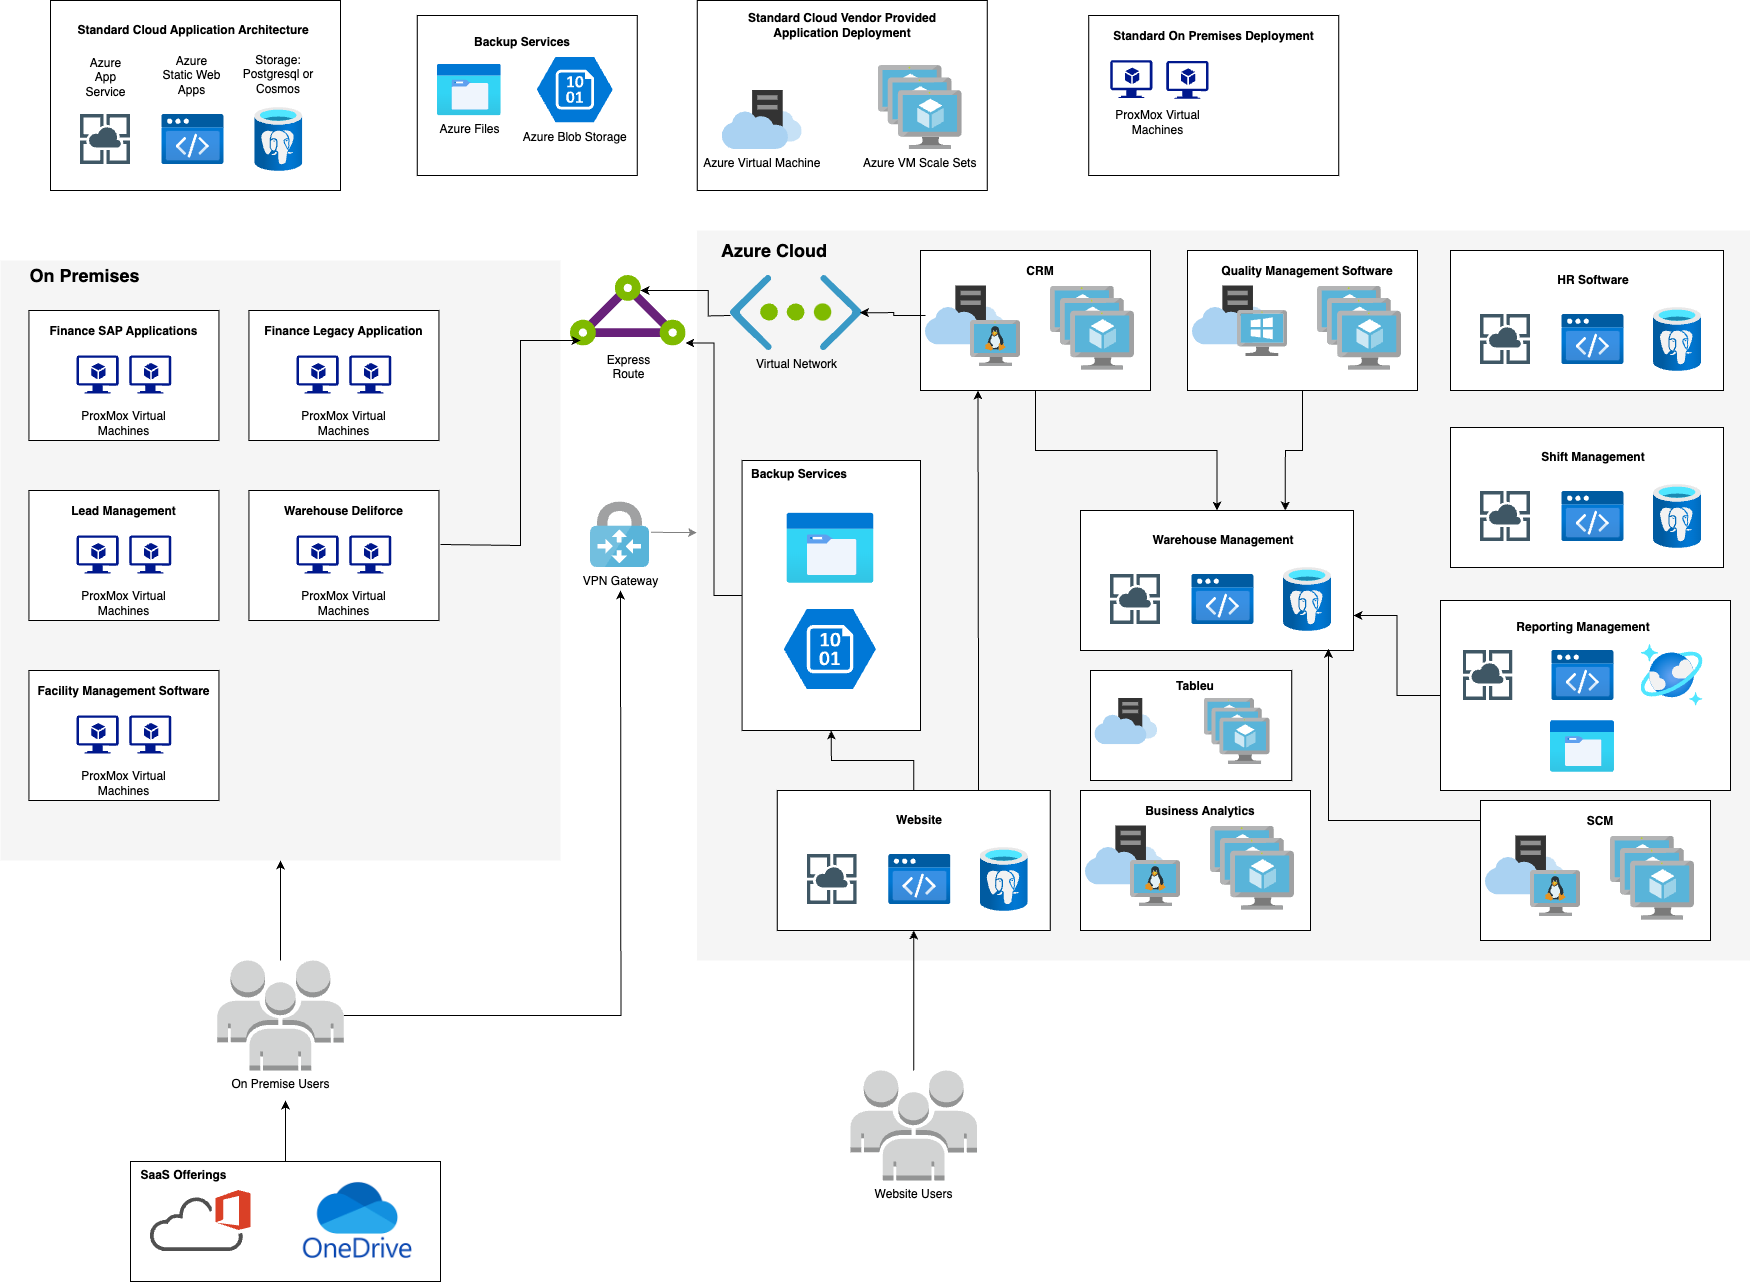
\includegraphics[width=1\textwidth]{diagrams/AzureArchCloud.png}
        \vspace{0.01\textwidth}
        \caption{Hybrid Cloud Architecture (Azure and On-Premises)}
        \label{Cloud_Architecture} % A unique label.
    \end{center}
\end{figure}

\subsection{Public Cloud Service Provider: Microsoft Azure}
\subsubsection{Azure App Service: PaaS} \leavevmode\newline
Azure App Service is a comprehensive HTTP-based  Platform-as-a-Service (PaaS) offering for developers, providing a fully managed environment for building, deploying, and scaling web applications under the offered service plan.

All the newly developed Python3 applications (Reporting Management, Shift Management, Warehouse Management, HR Software, and Webshop Website) will be deployed within the single Azure app service plan to optimize cost and performance, provided the plan has sufficient resources to handle the load as multiple apps in the same app service plan share the same VM instances.

\begin{itemize}
    \item \textbf{Service Plan:} \textit{Premium v3} - The premium service plan offers better compatibility with our application landscape and requirements compared to other tiers.
    \item Key features of this service
          \begin{itemize}
              \item \textbf{Auto-scaling \& Per-app scaling} - With automatic scaling enabled, Azure will monitor the load on your apps and distribute instances based on the metrics set up as such CPU usage. It also supports per-app scaling, allowing each app to scale independently based on its specific load.
              \item \textbf{Availability \& Zone Redundancy} - Azure SLA guarantees 99.95\% availability but in case case of availability zone failures it is advised to configure the app service plan as zone redundant, which means that your resources are spread across multiple availability zones. (Note: To enable zone redundancy at least 3 instances should be there in an app service plan).
              \item \textbf{Security} - Supports authentication, and IP address restriction and also offers virtual network integration.
              \item \textbf{Load-balancing} - Distributes incoming traffic across multiple instances to maximize throughput, minimize response time, and avoid overloading any single resource.
              \item \textbf{Multi-tenant} - Multiple clients can access the solution via their own individual domains.
          \end{itemize}

    \item \textbf{Operating System:} \textit{Linux} - Linux is the only operating system option for running Python apps in App Service. Linux is generally recommended due to better performance and compatibility with Python libraries
          .Linux also offers a more native environment for Python development\cite{azure-python}.

    \item \textbf{VM Instance:} \textit{P2v3} - \#Instances: 3

          \begin{itemize}
              \item \textbf{Core:} \textit{4}
              \item \textbf{RAM:} \textit{16}
              \item \textbf{Storage:} \textit{250 GB}
          \end{itemize}
\end{itemize}

\subsubsection{Azure Static Web App: PaaS} \leavevmode\newline
Azure Static Web Apps is a Platform-as-a-Service (PaaS) offering that automatically builds and deploys modern web apps with a static front-end to Azure from a code repository and provides seamless backend connection options.
Here, we will deploy our React.js based front for all newly developed applications to static web apps connected with dedicated Web apps from the App service plan explained above.
\begin{itemize}
    \item \textbf{Service Plan:} \textit{Standard} - \#Apps: 5

          \begin{itemize}
              \item \textbf{Included Bandwidth:} \textit{100 GB}
                    \textit{NOTE: We need 500 GB bandwidth}
              \item \textbf{Storage:} \textit{2 GB/app}
          \end{itemize}

    \item Key features of this service
          \begin{itemize}
              \item \textbf{Global Distribution} - static assets are distributed around the world, making serving files much faster as files are physically closer to end users.
              \item \textbf{DevOps \& CICD Pipeline} - Automated deployment from code repositories like GitHub or Azure DevOps based on code changes and allows CI/CD pipeline integration.
              \item \textbf{Security} - Supports authentication and Custom Domains with SSL certificates which are automatically renewed.
          \end{itemize}
\end{itemize}


\subsubsection{Microsoft Entra ID : PaaS} \leavevmode\newline
Microsoft Entra ID is a cloud-based identity and access management service that enables your employees to access cloud resources. Microsoft Entra ID Free edition is included with Azure cloud services (here, App Service \& Static Web Apps) which
provides security standards with multi-factor authentication.
It offers basic RBAC user and group management as well but advanced security is offered in paid plans only.

\subsubsection{Virtual Machine Scale Sets: IaaS} \leavevmode\newline
Azure Virtual Machine Scale Sets are a computing resource that allows the deployment and management of a set of identical, auto-scaling virtual machines.
We will be using it to manage our group of VMs. This service is offered free of cost along with the VM.
\begin{itemize}
    \item Key features of this service
          \begin{itemize}
              \item \textbf{Automatic scaling} -  Can automatically increase or decrease the number of VM instances based on demand or a defined schedule.
              \item \textbf{High availability} - Distributes VMs across fault domains and updates domains to ensure application resilience.
              \item \textbf{Load balancing} - Integrated with Azure Load Balancer for distributing traffic across VM instances.
          \end{itemize}
\end{itemize}

\subsubsection{Virtual Machine: IaaS} \leavevmode\newline
A total of 5 instances of VMs mentioned below will be deployed under 1 Scale Set for CRM application used by Operations, Sales \& Customer Service, and SCM used by Supply Management.
\begin{itemize}
    \item \textbf{CRM \& SCM} - \#Instances: 5
          \begin{itemize}
              \item \textbf{Instance:} \textit{Dpsv6}
              \item  \textbf{Operating System:} \textit{Ubuntu Linux}
              \item  \textbf{vCPUs:} \textit{2}
              \item  \textbf{RAM:} \textit{8 GiB}
          \end{itemize}
    \item \textbf{QM} - \#Instances: 1
          \begin{itemize}
              \item \textbf{Instance:} \textit{Dpsv6}
              \item  \textbf{Operating System:} \textit{Windows}
              \item  \textbf{vCPUs:} \textit{2}
              \item  \textbf{RAM:} \textit{8 GiB}
          \end{itemize}
    \item Key features of this service
          \begin{itemize}
              \item  \textbf{New optimised architecture:} \textit{Outstanding performance for general-purpose workloads for day-to-day business operations.}
              \item  \textbf{Balanced performance:} \textit{Equipped with faster processors provides a solid balance between CPU capabilities and memory size.}
          \end{itemize}
\end{itemize}

\subsubsection{Azure Database(PostgreSQL/Cosmos DB) : PaaS} \leavevmode\newline
In the newly adjusted application landscape no specific details of the database so we will assume the size of the database's previous application landscape.

\begin{itemize}
    \item \textbf{Azure PostgreSQL}
          \begin{itemize}
              \item \textbf{Payroll:} \textit{1 TB - used by HR Software and Shift Management}
              \item  \textbf{Delivery:} \textit{250 GB - used by Warehouse Management}
              \item  \textbf{CRM:} \textit{980 GB - used by Sales, Operation and Customer Service}
              \item  \textbf{CMS:} \textit{10 GB - used by Webshop Website}
          \end{itemize} \leavevmode\newline
          The chosen configuration for our solution is mentioned below.
          \begin{itemize}
              \item \textbf{Server:} \textit{D2ds v5 - Flexible}
              \item  \textbf{vCores:} \textit{2}
              \item  \textbf{Memory:} \textit{8 GiB}
              \item  \textbf{Storage:} \textit{Premium SSD v2 configuration - 2240 GB \textasciitilde 2085 GiBs}
              \item  \textbf{IOPS:} \textit{3000 at no additional cost, Our estimated requirement is \textasciitilde 6000}
              \item  \textbf{Provisioned Throughput:} \textit{125 MB/S}
              \item  \textbf{Backup Storage:} \textit{Geo-Redundant Storage (GRS) - 2240 GB \textasciitilde 2085 GiBs}
          \end{itemize}
    \item Key features of this service
          \begin{itemize}
              \item  \textbf{Flexibility:} \textit{Fully managed database service offering more control and flexibility over database management and configuration.}
              \item  \textbf{Balanced performance:} \textit{Balanced compute and storage capacities with scalable I/O throughput, efficient cost-performance ratio}
              \item  \textbf{High availability \& Low latency:} \textit{Allows users to collocate the database engine with the client tier for lower latency and choose high availability within a single availability zone or zone redundant (At extra cost)}
              \item  \textbf{Redundancy:} \textit{The storage maintains three locally redundant synchronous copies of the database files ensuring data durability.}
              \item  \textbf{Backup:} \textit{GRS replicates your data in a secondary region several hundred kilometers away from the primary source data location and provides greater durability of your data even in the event of a regional outage.}
          \end{itemize}
    \item \textbf{Azure CosmosDB}
          \begin{itemize}
              \item \textit{Reporting Management - Details not mentioned}

          \end{itemize}
\end{itemize}

\subsubsection{Azure Storage : IaaS} \leavevmode\newline
\begin{itemize}
    \item \textbf{Managed Disk} - \textit{Needed to use with Azure VM for CRM, SCM, and QM for both the VM Scale sets}
    \item \begin{itemize}
              \item \textit{Standard SSD}
              \item  \textbf{Storage:} \textit{2048 GiB + 128 GiB}
              \item  \textbf{IOPS:} \textit{500}
              \item  \textbf{Provisioned Throughput:} \textit{100 MB/S}
              \item  \textbf{Backup:} \textit{LRS (Locally redundant storage)}
          \end{itemize}
    \item \textbf{Blob Storage: Hot} - \textit{For storing reports in Reporting Management}
    \item \begin{itemize}
              \item  \textbf{Storage:} \textit{512 GiB}
              \item  \textbf{Redundancy:} \textit{LRS (Locally redundant storage)}
          \end{itemize}
    \item \textbf{Azure Files} - \textit{For Legacy Application storage}
    \item \begin{itemize}
              \item  \textbf{Service Plan:} \textit{SSD - Provisioned v1}
              \item  \textbf{Storage:} \textit{256 GiB}
              \item  \textbf{Redundancy:} \textit{LRS (Locally redundant storage)}
          \end{itemize}
\end{itemize}
\section{Cost of operations in Microsoft Azure (Excluding Software Licensing) \cite{azure-pricing-calculator}}
\begin{table}[htbp]
    \centering
    \begin{tabular}{|l|c|c|c|c|}
        \hline
        \textbf{Azure Cloud Service} & \textbf{Plan Details} & \textbf{Cost/Month}                  & \textbf{Quantity} & \textbf{Total Cost/Month}           \\

        \hline
        App Service                  & 3 years savings plan  & \textasciitilde 136 €                & 3                 & ~\textasciitilde 408 €              \\
        \hline
        Static Web Apps              & Standard              & \textasciitilde 8.5 € + (0.191 €/GB) & 5 + (500 GB)      & 43 € + 95 € = \textasciitilde 138 € \\
        \hline
        Virtual Machine              & Dpsv6                 & \textasciitilde 27 €                 & 6                 & \textasciitilde 162 €               \\
        \hline
        Database - Server            & D2ds v5 - Flexible    & \textasciitilde 59 €                 & 1                 & \textasciitilde 59 €                \\
        \hline
        Database - Storage           & SSD Premium v2        & \textasciitilde 0.13 €/GiB           & 2085              & \textasciitilde 274 €               \\
        \hline
        Database - Additional IOPS   & Additional            & \textasciitilde 0.02 €               & 3000              & \textasciitilde 75 €                \\
        \hline
        Database - Backup Storage    & GRS - additional cost & \textasciitilde 0.099 €              & 1000              & \textasciitilde 99 €                \\
        \hline
        Storage                      & SSD Standard          & \textasciitilde 147 € + 9 €          & 1                 & \textasciitilde 156 €               \\
        \hline
        Blob Storage                 & Hot                   & \textasciitilde 0.0189 €/GB          & 512               & \textasciitilde 10 €                \\
        \hline
        Azure Express Route          & 50 Mbit/s             & \textasciitilde 52 €                 & 1                 & \textasciitilde 52 €                \\
        \hline
        Azure Files                  & SSD - Provisioned v1  & \textasciitilde 47 €                 & 1 (256 GB)        & \textasciitilde 47 €                \\
        \hline
        Tableau                      &                       & \textasciitilde                      &                   & \textasciitilde                     \\
        \hline
        \textbf{Total Cost:}         & -                     & -                                    &                   & \textbf{1480  €}                    \\
        \hline
    \end{tabular}
    \caption{Cost of operations in Microsoft Azure}
    \label{tab:Cost_Operation_Monthly}
\end{table}


\section{Cloud Migration Roadmap}

For the migration we have determined 4 different workstreams:
\begin{enumerate}
    \item New Application Development
    \item COTS Applications Cloud Installation
    \item On Premises Deployments
    \item SaaS Sourcing and Configuration
\end{enumerate}

\subsubsection{New Application Development}
In this case the majority of the effort is in the development process, we are estimating at least 12 months of development time. An advantage of the "new application standard" is that we are shipping continuously.
This means that from the first line of code, the application is deployed to the cloud and accessible. We plan for several teams to work in different applications concurrently.

\subsubsection{COTS Applications Cloud Installation}
For Cloud Installations we are focusing on creating the infrastructure as code files, and the subsequent deployments to Azure. This applications will be usable as soon as the installation ins completed. Given that all other dependencies are accessible.

\subsection{On Premises Deployments}

Similar to the cloud deployments, we are focusing on creating Ansible playbooks and the relevant ProxMox configurations. These applications will be usable once the deployment ins completed.

\subsection{Saas Sourcing and Configuration}

In this case we are interested on enrolling for the software, configuring access policies and potentially negotiating enterprise licenses with the providers. This is the shortest phase and users will be able to use the applications once licences and credentials are available.

\begin{figure}[htbp]
    \begin{center}
        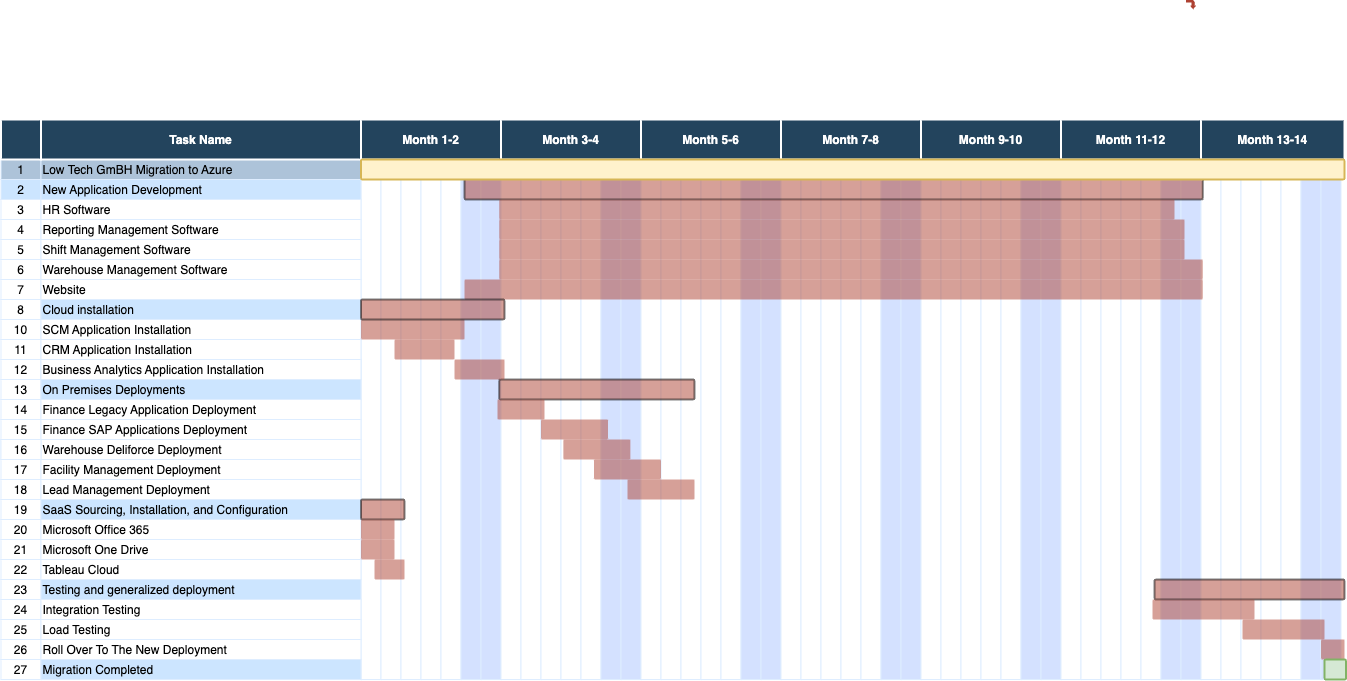
\includegraphics[width=1\textwidth]{diagrams/roadmap.png}
        \vspace{0.01\textwidth}
        \caption{Visualised Cloud Migration Roadmap}
        \label{cloud migration roadmap} % A unique label.
    \end{center}
\end{figure}


\section{Standard For a Cloud Native Application}

When developing a cloud-native application Figure \ref{CloudStandard} shows the basic setup to integrate DevOps concepts into our workflow.
The website is going to be developed under this standard.\\

\begin{figure}[htbp]
    \begin{center}
        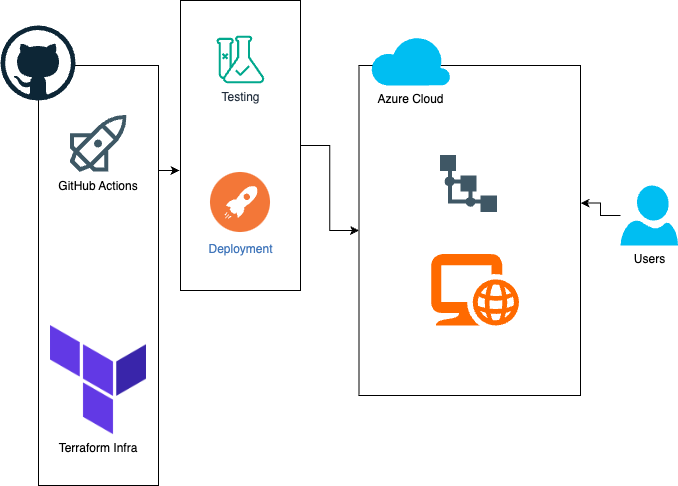
\includegraphics[width=0.5\textwidth]{diagrams/AppStandard.drawio.png}
        \vspace{0.01\textwidth}
        \caption{Standard Configuration To Deploy An Application}
        \label{CloudStandard} % A unique label.
    \end{center}
\end{figure}
\newpage
\subsection*{Contribution}

\begin{table}[htbp]

    \begin{tabular}{|p{0.7\textwidth}|p{0.3\textwidth}|}
        \hline
        \textbf{Topic}                             & \textbf{Contributor}                    \\
        \hline
        1. Overview of the Problem \newline
        2. Objectives of the Migration             & Priyanka Vadiwala                       \\
        \hline
        3. Migration Strategy \newline
        7. Standard For a Cloud Native Application & Wladymir Brborich-Herrera               \\
        \hline
        4. Proposed Cloud Architecture \& Justfication of Used Service Models \newline
        5. Cost of operations in Microsoft Azure   & Hellyben Shah  \newline  Heer Vankawala \\
        \hline
        6. Cloud Migration Roadmap                 & Vishwaben kakadiya                      \\
        \hline
    \end{tabular}
    \caption{Contribution Table}
    \label{tab:contribution}
\end{table}

% ---- Bibliography ----

\begin{thebibliography}{5}

    \bibitem{MicrosoftAzureHostingPlans}
    Microsoft,
    \emph{Azure App Service plan overview},
    2024, Available:
    \url{https://learn.microsoft.com/en-us/azure/app-service/overview-hosting-plans}.

    \bibitem{MicrosoftAzureSubscriptionLimits}
    Microsoft,
    \emph{Azure subscription and service limits, quotas, and constraints},
    2024, Available:
    \url{https://learn.microsoft.com/en-us/azure/azure-resource-manager/management/azure-subscription-service-limits}.

    \bibitem{azure-pricing-calculator}
    Microsoft, Available:
    \emph{Azure Pricing Calculator}, 2024,
    \url{https://azure.microsoft.com/de-de/pricing/calculator/}.



\end{thebibliography}
\end{document}
